\documentclass{article}
\usepackage[utf8]{inputenc}
\usepackage[brazil]{babel}
\usepackage{graphicx}
\usepackage{fancyvrb}
\bibliographystyle{ieeetr}

\title{Ferramenta Web para Visualização de DSM\\
 \large MATE26 - Tópicos Especiais em Engenharia de Software II (2013.1)}
\author{
  Joenio Marques da Costa\\
  \texttt{joenio@colivre.coop.br}
  \and
  Daniela Soares Feitosa\\
  \texttt{daniela@colivre.coop.br}
}
\date{07 de junho de 2013}

\begin{document}

\maketitle

Este trabalho visa o desenvolvimento de uma interface Web para visualização de
{\it Design Structure Matrices (DSM)} com base na ferramenta {\it
Analizo}\footnote{http://analizo.org}, um conjunto de ferramentas para análise
e visualização de código fonte extensível e independente de linguagem.

{\it DSM} é uma ferramenta que destaca a estrutura inerende de um design de um
produto ou projeto examinando as dependencias existentes entre seus
componentes através de uma matrix simétrica\cite{ExploringStructure}. Ela foi
inicialmente  (Steward, 1981) proposta no contexto de gestão de projetos com
objetivo de melhorar o fluxo de informações entre tarefas e atividades, e tem
sido utilizada constantemente com este objetivo como visto em
\cite{AModelBasedMethod}

Desde então tem sido utilizado nos mais variados contextos
\cite{PredictingChange, PredictingRequirementChange, UsingTheDesignStructure}
incluindo as áreas de engenharia de software, compreensão, visualização,
análise de impacto, dentre outras.  Uma grande vantagem da visualização de
software através de DSM é que ela consegue exibir uma grande quantidade de
informação em uma forma compacta, assim é possível demonstrar arquitetura de
softwares complexos com muitos elementos interelacionados de forma
compacta\cite{DependencyModel}.

DSMs podem ser utilizada para identificar possíveis formas de reorganizar os
elementos de um sistema a fim de reduzir custos de coordenação, facilitando o
fluxo de informações entre os elementos. Elementos com um alto nível de
dependencia são agrupados em cluster ou módulos.

Para guiar este processo uma gama de algoritmos de clusterizing tem sido
desenvolvidos, com objetivo de minimizar custo de coordenação, este trabalho
tem como objetivo implementar ao menos um desdes algoritmos na ferramenta {\it
Analizo}.

\begin{figure}[h]
\center
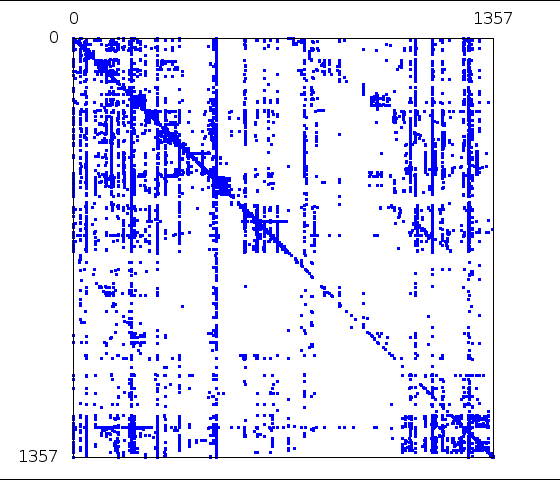
\includegraphics[scale=0.5]{linux.png}
\caption{Design Structure Matrix do Linux 2.0 gerado pelo Analizo}
\label{fig:dsm}
\end{figure}

O {\it Analizo} já possui suporte a construção de DSM de projetos de software
escritos em C, C++ ou Java, como pode ser visto na Figura~\ref{fig:dsm}.

Contudo a visualização de DSM provida pelo {\it Analizo} é estática e não
oferece nenhuma interação com o usuário, este trabalho visa evoluir esta
funcionalidade provendo:

\begin{itemize}
  \item Interface Web para visualização de DSM
  \item Implementação de algoritmos de clusterização de DSM
  \item Interação com zoom e reorganização da DSM em clusters
\end{itemize}

Deverá ser possível através da interface Web selecionar uma entre várias
sugestões de organização da DSM em cluster calculada automaticamente pela
ferramenta. A organização padrão será cluster com base na organização de
diretórios dada ao projeto pelos seus desenvolvedores.

Esta ferramente irá prover ainda a infraestrutura para que usuários cadastrem
endereços de repositórios de código-fonte que serão então automaticamente
copiados para serem então analizados e disponibilizados para visualização e
interação com a DSM.

Outras referências sobre DSMs:
\cite{AKnowledgeBased, AnalyzingTheEvolution, AntaresDSM, ApplyingTheDesign,
DesignSuite, EfficientOrganizing, ReachabilityMatrices, TheStructureAndValue}.

% TODO pesquisar tais artigos:
% Compreensão e Visualização de Projetos Orientados a Objetos com Matriz de Dependências
% A design structure matrix (dsm) aplicada ao projeto de navios
% Procurar artigo de Steward, 81

\bibliography{bibliografia}
\end{document}
